\documentclass[10pt,a4paper]{article}
\usepackage[utf8]{inputenc}
\usepackage[T1]{fontenc}
\usepackage[provide=*,spanish]{babel}
\usepackage[margin=1.65cm,top=1.6cm,bottom=1.65cm]{geometry}
\usepackage{lmodern,microtype,amsmath,amssymb,booktabs,tabularx,graphicx,xcolor,enumitem,fancyhdr,titlesec}
\usepackage{xurl}
\usepackage[hidelinks]{hyperref}
\hypersetup{pdftitle={Práctica 01 - Búsquedas y Notación Asintótica},pdfauthor={Yana Mendoza; Belizario Yana; Curasi Zevallos}}
\definecolor{azul}{HTML}{164A65}
\titleformat{\section}{\large\bfseries\color{azul}}{\thesection.}{.5em}{}
\titlespacing*{\section}{0pt}{7pt}{3pt}
\setlength{\parindent}{0pt}
\setlength{\parskip}{4pt}
\setlist{nosep,leftmargin=*}
\pagestyle{fancy}\fancyhf{}
\fancyhead[L]{\small SIS210 · Búsquedas y Notación Asintótica}
\fancyhead[R]{\small UNA -- Puno}
\fancyfoot[C]{\small\thepage}
\setlength{\headheight}{13pt}
\newcommand{\VentajaBinariaCpp}{1236.0}
\newcommand{\PenalidadInterpolacionCpp}{45.1}
\newcommand{\CrecimientoLinealCpp}{46.7}
\newcommand{\VentajaInterpolacionCpp}{14.4}
\newcommand{\VentajaBinariaPy}{2756.4}
\newcommand{\PenalidadInterpolacionPy}{36.7}
\newcommand{\CrecimientoLinealPy}{49.9}
\newcommand{\VentajaInterpolacionPy}{11.3}
\begin{document}
\hypersetup{pageanchor=false}\begin{titlepage}
\centering
\vspace*{1.7cm}
{\Large\bfseries UNIVERSIDAD NACIONAL DEL ALTIPLANO\par}
\vspace{.3cm}{\Large Puno\par}
\vspace{.7cm}{\large Escuela Profesional de Ingeniería de Sistemas\par}
\vspace{1.9cm}
{\color{azul}\rule{\textwidth}{1pt}\par}
\vspace{.5cm}
{\LARGE\bfseries Práctica 01 — Búsquedas y\par Notación Asintótica\par}
\vspace{.4cm}
{\large Implementación y comparación experimental en Python y C++\par}
\vspace{.5cm}{\color{azul}\rule{\textwidth}{1pt}\par}
\vspace{1.5cm}
{\large\textbf{Curso}\par Algoritmos y Estructuras de Datos -- SIS210\par}
\vspace{.8cm}
{\large\textbf{Docente}\par ZANABRIA GALVEZ ALDO HERNAN\par}
\vspace{.8cm}
{\large\textbf{Integrantes}\par}
\vspace{.2cm}
YANA MENDOZA CARLOS BENEDICTO\par
BELIZARIO YANA DAVID VICTOR\par
CURASI ZEVALLOS HANDDY RONALD\par
\vfill
{\large Puno -- Perú\par 2026\par}
\vspace{.5cm}
\end{titlepage}
\hypersetup{pageanchor=true}\setcounter{page}{1}
\tableofcontents\clearpage
\section{Estado del arte y marco teórico ampliado}
\subsection{Núcleo 1. Problema de búsqueda, contrato y representación}
Una búsqueda debe definirse antes de medirla: dada una secuencia $a$ de longitud $n$ y una clave $x$, se pide devolver un índice válido que cumpla $a[i]=x$, o informar ausencia. El contrato distingue la operación abstracta de su implementación y evita confundir pertenencia con recuperación de la primera aparición. Morin (s.\,f., sección 1.2) desarrolla esta separación mediante interfaces; Sedgewick y Wayne (2011, sección 1.1) presentan la búsqueda sobre arreglos como una operación concreta; Erickson (2019, capítulo 0) exige especificaciones precisas para argumentar corrección. En esta práctica, cuando existen duplicados, cualquier coincidencia satisface el contrato: dos índices distintos pueden ser igualmente correctos.

La representación condiciona qué estrategias son aplicables. Un arreglo ofrece posiciones indexadas; una fuente secuencial obliga a consumir elementos anteriores para alcanzar los siguientes. Morin (s.\,f., sección 1.4) explicita el modelo de acceso, mientras Sedgewick y Wayne (2011) conectan la representación con las operaciones del programa. La perspectiva de diseño de Skiena (2020) ayuda a formular la decisión práctica: primero reconocer las restricciones y después elegir la técnica. Aplicado aquí, el certificado de orden es información útil, pero su ausencia no puede reemplazarse por una suposición. Buscar correctamente en una lista desordenada y buscar rápidamente en una lista ya ordenada son contratos de entrada diferentes, aunque ambos devuelvan un índice.

\textbf{Aplicación razonada.} Para $a=[4,4,9]$ y $x=4$, los índices 0 y 1 son válidos; para $x=7$ solo lo es $-1$. La comprobación usada por el proyecto refleja exactamente esta condición. No exige índices idénticos entre algoritmos como requisito general de correctitud.

\subsection{Núcleo 2. Modelo RAM, operaciones y costo espacial}
El modelo RAM permite estudiar el número de operaciones sin fijar primero una velocidad de procesador. Se supone acceso a una palabra de memoria y operaciones elementales con costo acotado. Morin (s.\,f., sección 1.4) precisa el modelo \emph{word-RAM}; el enfoque de Cormen et al. (2022) proporciona el marco del análisis de algoritmos, y Sedgewick y Wayne (2011, sección 1.4) distinguen frecuencia y costo de las instrucciones. Esta abstracción hace comparable el trabajo de dos procedimientos, pero no afirma que una división, una comparación y un acceso real a memoria duren lo mismo. El conteo necesita declarar qué considera operación y qué información deja fuera.

La memoria auxiliar también debe separarse del tamaño de entrada. Las cuatro versiones iterativas conservan un número constante de índices y variables, por lo que utilizan $O(1)$ palabras auxiliares; almacenar el arreglo y las consultas exige memoria adicional. Morin (s.\,f., sección 1.5) diferencia recursos de representación y operación; Erickson (2019) advierte que el análisis depende del modelo, y la documentación de Python describe enteros con precisión no limitada a una palabra fija (Python Software Foundation, s.\,f.-a). Por ello, el supuesto de aritmética constante se aplica aquí a las magnitudes acotadas del experimento: no debe extrapolarse a enteros arbitrariamente grandes. En C++, además, se amplía el cálculo antes de restar y multiplicar para evitar desbordamientos en la interpolación de estas entradas.

\textbf{Aplicación razonada.} Guardar $\ell$, $h$ y $m$ no multiplica la memoria auxiliar por $n$. En cambio, copiar el arreglo para ordenarlo sí introduce almacenamiento proporcional a $n$. El cronómetro del proyecto excluye esa preparación, de modo que sus tiempos no son el costo de una solución completa que primero deba ordenar.

\subsection{Núcleo 3. Significado y uso correcto de \texorpdfstring{$O$, $\Omega$ y $\Theta$}{O, Omega y Theta}}
La notación asintótica describe cotas de crecimiento, no unidades de tiempo. Para funciones no negativas, $T(n)\in O(g(n))$ si existen $c>0$ y $n_0$ tales que $T(n)\leq c g(n)$ para todo $n\geq n_0$; $\Omega$ invierte la desigualdad y $\Theta$ exige ambas cotas. El tratamiento de Cormen et al. (2022), el trasfondo matemático de Morin (s.\,f., sección 1.3) y el análisis de recurrencias de Erickson (2019) son complementarios: una cota solo tiene sentido cuando se define la función analizada. Escribir $O(n)$ no significa que se ejecuten exactamente $n$ comparaciones ni que el tiempo se duplique con precisión al duplicar una entrada concreta.

Para comparar búsquedas interesa una cota ajustada cuando pueda justificarse. Por ejemplo, $3n+7$ pertenece a $\Theta(n)$ y también a $O(n^2)$, pero la segunda afirmación comunica menos. La distinción entre cota válida y descripción informativa se apoya en Morin (s.\,f.), Cormen et al. (2022) y Erickson (2019); la aplicación algebraica siguiente es una elaboración propia. Para $n\geq1$, $3n\leq3n+7\leq10n$, por lo que existen las dos cotas lineales. Asimismo, cambiar la base de $\log n$ solo multiplica por una constante. Sin embargo, $\log\log n$ no puede reemplazarse por una constante en un análisis general, aunque cambie muy lentamente en los tres tamaños medidos.

\textbf{Consecuencia para el informe.} Las mediciones finitas pueden ser compatibles con una función de crecimiento; no establecen por sí mismas una desigualdad válida para todos los tamaños futuros. Una demostración asintótica necesita un argumento sobre el algoritmo, no solo puntos en un gráfico.

\subsection{Núcleo 4. Mejor caso, promedio, peor caso y mezcla de consultas}
Los casos y las notaciones responden preguntas diferentes. El mejor caso minimiza el costo entre entradas de tamaño $n$; el peor lo maximiza; el promedio pondera los costos mediante una distribución explícita. Morin (s.\,f., sección 1.5) distingue garantías y expectativas; Erickson (2019) explica por qué un argumento debe cubrir las entradas admitidas, y Sedgewick y Wayne (2011, sección 1.4) señalan la dependencia del rendimiento respecto de la entrada. Por tanto, $\Omega$ no es un sinónimo de mejor caso ni $\Theta$ de promedio. Una búsqueda binaria puede tener mejor caso $\Theta(1)$ y peor caso $\Theta(\log n)$ sin que exista contradicción.

La mezcla 70/30 de esta práctica define una carga concreta: 70\% de aciertos y 30\% de ausencias. El promedio observado depende también de qué posiciones y qué claves ausentes se seleccionan. La necesidad de explicitar distribuciones se relaciona con Sedgewick y Wayne (2011), el análisis probabilístico de Morin (s.\,f., sección 1.3) y la dependencia de la distribución estudiada por Van Sandt et al. (2019). El modelo propio para lineal, con claves únicas y hits equiprobables por posición, produce
\[
E[C]=0.7\frac{n+1}{2}+0.3n=0.65n+0.35.
\]
No es un nuevo resultado experimental: es una expectativa teórica con la cual interpretar el conteo existente. Los duplicados y el retorno de la primera coincidencia pueden modificarla.

\textbf{Lectura crítica.} Un miss por encima del máximo puede descartarse inmediatamente en interpolación, mientras lineal recorre todo el arreglo. Cambiar la ubicación de los misses manteniendo el 30\% puede cambiar el tiempo promedio. La proporción por sí sola no describe completamente el experimento.

\subsection{Núcleo 5. Correctitud, invariantes y terminación}
Una implementación eficiente debe primero satisfacer su contrato. La correctitud parcial establece que la respuesta es válida si termina; la terminación completa el argumento. Erickson (2019, capítulo 0) presenta el razonamiento de corrección, Morin (s.\,f., sección 1.5) lo distingue del costo y Sedgewick y Wayne (2011, sección 1.1) ofrecen la búsqueda binaria como programa verificable. En las búsquedas por intervalo, un invariante apropiado es: si la clave está presente y aún no fue encontrada, permanece entre los límites activos. Esta formulación permite explicar cada descarte en vez de confiar en que un conjunto de ejemplos haya funcionado.

Para binaria, el orden permite conservar el invariante al descartar la mitad incompatible con la comparación central; actualizar a $m+1$ o $m-1$ hace disminuir el intervalo. Para interpolación también debe garantizarse avance, aunque su estimación no divida por la mitad. Esta aplicación combina el esquema de prueba de Erickson (2019), la especificación de algoritmos de Sedgewick y Wayne (2011) y la estimación por valores de Perl et al. (1978). En el proyecto, el vacío se controla antes de indexar y la igualdad de extremos antes de dividir. Las pruebas existentes aportan evidencia de implementación; el razonamiento sobre invariantes explica por qué las actualizaciones son válidas para toda entrada que cumpla las precondiciones.

\textbf{Ejemplo de fallo evitado.} Si se escribiera $\ell=\text{pos}$ y la estimación repitiera el mismo índice, el intervalo podría no reducirse. Usar $\ell=\text{pos}+1$ elimina una posición ya comprobada y garantiza progreso. Esta explicación no modifica el código entregado.

\subsection{Núcleo 6. Búsqueda lineal como referencia y solución práctica}
Lineal compara sucesivamente la clave con cada elemento y termina al encontrar una coincidencia. El recorrido directo encaja en el modelo de operaciones de Morin (s.\,f.) y en el análisis de programas de Sedgewick y Wayne (2011); Skiena (2020) aporta la perspectiva de elegir una solución según las restricciones reales. Su ventaja estructural es que no exige preparación ni orden. En el peor caso debe revisar los $n$ elementos: cualquier posición todavía no inspeccionada podría contener la clave. Esta necesidad ofrece una justificación del costo lineal para el problema sin información adicional, no solamente una observación sobre el ciclo \texttt{for}.

El mejor caso ocurre en el primer elemento; una ausencia obliga a completar el recorrido y un hit intermedio depende de su posición. La interpretación conjunta del modelo de Morin (s.\,f.), las condiciones de búsqueda de Sedgewick y Wayne (2011) y los efectos de memoria de Van Sandt et al. (2019) evita descartar lineal por su notación. Para arreglos muy pequeños o pocas consultas, los gastos de preparación pueden superar el ahorro de una estrategia más elaborada. Sus accesos consecutivos favorecen localidad espacial, pero no eliminan el crecimiento de trabajo. En los tamaños evaluados, la reducción de comparaciones de binaria es suficientemente grande para prevalecer en datos ordenados; esta conclusión se limita a los resultados ya conservados.

\textbf{Derivación propia.} Si el acierto aparece en el índice $i$, lineal realiza $i+1$ igualdades; si no aparece, realiza $n$. Sumar esas cantidades para las consultas almacenadas explica el oráculo independiente usado en la auditoría original, sin necesitar volver a ejecutar el benchmark.

\subsection{Núcleo 7. Búsqueda binaria: reducción, recurrencia y garantía}
Binaria utiliza el orden para elegir un único subintervalo después de examinar su centro. Sedgewick y Wayne (2011, sección 1.1) documentan la condición de arreglo ordenado; Erickson (2019, capítulo 1) desarrolla el razonamiento recursivo y las recurrencias, y Morin (s.\,f., sección 1.3) proporciona el trasfondo logarítmico. La traducción propia a una recurrencia de peor caso es $T(n)=T(\lfloor n/2\rfloor)+\Theta(1)$, salvo ajustes de extremos. Después de $k$ reducciones quedan aproximadamente $n/2^k$ candidatos; alcanzar un intervalo de tamaño constante requiere $k$ proporcional a $\log_2n$. La versión iterativa implementa la misma reducción sin una pila recursiva.

La garantía depende del orden y no de la separación numérica entre claves. Esto diferencia a binaria de interpolación: grandes huecos no impiden descartar una mitad por índices. La comparación se apoya en el algoritmo de Sedgewick y Wayne (2011), la sensibilidad de interpolación de Perl et al. (1978) y el estudio práctico de Van Sandt et al. (2019). En el uniforme, el sesgado y los arreglos con repetidos se conserva la validez de binaria, aunque los duplicados alteren dónde termina. El mejor caso es encontrar la clave en el primer centro; para posiciones equiprobables y claves distintas, el promedio crece logarítmicamente. No se promete que cada búsqueda individual use exactamente $\log_2n$ comparaciones.

\textbf{Traza propia.} En $[2,4,8,12,18]$, buscar 12 examina primero 8 y luego 12. Buscar 7 termina con el intervalo vacío después de descartar posiciones incompatibles. Las dos trayectorias tienen costos distintos, aunque compartan algoritmo y tamaño.

\subsection{Núcleo 8. Búsqueda exponencial y límite efectivo desconocido}
Exponencial separa dos problemas: localizar una cota y buscar dentro de ella. El ejercicio de lanzamiento de huevos de Sedgewick y Wayne (2011, sección 1.4) propone duplicación repetida seguida de búsqueda binaria; el análisis de reducción de Erickson (2019) y los logaritmos de Morin (s.\,f.) permiten justificar el esquema empleado aquí. Tras resolver el índice cero, se prueban $1,2,4,8,\ldots$ hasta encontrar un valor no menor que $x$ o alcanzar el final. Para una posición objetivo $p\geq1$, se necesitan $O(\log p)$ ampliaciones; el intervalo resultante tiene tamaño $O(p)$ y su refinamiento binario también cuesta $O(\log p)$. Una forma uniforme que contempla el inicio es $O(1+\log(p+1))$.

Su utilidad depende de la interfaz. Morin (s.\,f., secciones 1.2 y 1.4) separa operaciones disponibles y representación; Sedgewick y Wayne (2011) vinculan búsqueda y acceso a arreglos, y Skiena (2020) destaca la adecuación del diseño al problema. Una fuente sin longitud inicial puede permitir \texttt{leer(i)} con una señal segura de fin; en ese caso tiene sentido duplicar índices. Un flujo exclusivamente secuencial no ofrece ese salto a costo constante. Nuestra implementación conoce $n$ y utiliza una cota finita: conserva el mecanismo, pero no mide la ventaja de desconocer el límite. Para claves lejanas, la fase adicional puede aportar comparaciones sin mejorar a binaria directa.

\textbf{Traza propia.} Si la primera posición con valor suficiente es 13, las sondas 1, 2, 4, 8 y 16 delimitan un intervalo que contiene esa posición. El refinamiento se aplica dentro de la cota, no sobre todos los índices desde cero.

\subsection{Núcleo 9. Interpolación y modelo de posición por valor}
Interpolación aprovecha información numérica que binaria no necesita. Estima la fracción del rango de valores ocupada por $x$ y la proyecta sobre el rango de índices. Perl et al. (1978) estudian la búsqueda bajo uniformidad, Van Sandt et al. (2019) revisan su comportamiento en memoria y Sedgewick y Wayne (2011) ofrecen binaria como término de comparación por índices. La fórmula implementada es
\[
\text{pos}=\ell+\left\lfloor\frac{(x-a[\ell])(h-\ell)}{a[h]-a[\ell]}\right\rfloor.
\]
Los límites de valor deben verificarse antes de calcularla. Si los extremos son iguales, el denominador desaparece y es necesario resolver ese caso por separado. Esta estimación es un modelo de la distribución, no una posición garantizada.

El esperado $O(\log\log n)$ pertenece a un modelo probabilístico de claves uniformes; no es una garantía para toda secuencia ordenada. El vínculo con ese supuesto proviene de Perl et al. (1978), la degradación práctica se analiza en Van Sandt et al. (2019) y la distinción entre esperado y peor caso aparece en Morin (s.\,f., sección 1.5). En nuestra entrada consecutiva $a[i]=i$, sustituir en la fórmula da exactamente $\text{pos}=x$ para un hit dentro del rango. Esa deducción propia explica el comportamiento especialmente favorable ya observado. No demuestra que toda muestra aleatoria uniforme se resuelva en un paso ni autoriza a reemplazar la cota esperada general por $O(1)$.

\textbf{Caso adverso razonado.} En $[0,1,\ldots,n-2,n^2]$ buscando $n-2$, el valor extremo agranda mucho el denominador. Las estimaciones avanzan casi de una posición en una, de modo que puede aparecer un costo $\Theta(n)$. Este ejemplo analítico no se agregó a los datasets ni se presenta como un experimento nuevo.

\subsection{Núcleo 10. Distribución, duplicados y selección de hits y misses}
La distribución relevante relaciona valores con posiciones, no solo el hecho de que la secuencia esté ordenada. La hipótesis uniforme de Perl et al. (1978), el análisis de datos no uniformes de Van Sandt et al. (2019) y los modelos de entrada de Sedgewick y Wayne (2011) explican por qué debe describirse el generador. En el sesgado del proyecto, muchas posiciones corresponden a un intervalo numérico pequeño. La fracción $(x-a[\ell])/(a[h]-a[\ell])$ puede entonces subestimar la fracción de posiciones hasta $x$. Binaria sigue dividiendo por índices; interpolación necesita corregir estimaciones que responden a una densidad local muy diferente de la global.

Los duplicados y la elección de consultas añaden otra capa. Morin (s.\,f., sección 1.2) obliga a precisar la operación solicitada, Sedgewick y Wayne (2011) advierten la dependencia de la entrada y la documentación de Python distingue muestreo y control pseudoaleatorio (Python Software Foundation, s.\,f.-b). Elegir hits por posición hace que los valores repetidos tengan mayor probabilidad de ser consultados: no equivale a muestrear uniformemente las claves distintas. Por otra parte, los misses originales se encuentran por encima del máximo, de modo que su descarte es especialmente sencillo para interpolación. Son propiedades del protocolo conservado; se explicitan para limitar el alcance de la interpretación, no para sustituir la carga por otra más favorable.

\textbf{Lectura del sesgo.} Tener exactamente 80\% de valores en el rango estrecho garantiza la composición del dataset, pero no garantiza exactamente 80\% de los 700 hits en ese rango. Los hits se muestrean con reemplazo y su composición particular depende de la semilla.

\subsection{Núcleo 11. Rendimiento real, instrumentación y reproducibilidad}
Un tiempo medido incluye el costo de ejecutar instrucciones sobre un entorno real. Sedgewick y Wayne (2011, sección 1.4) relacionan frecuencia y costo; Van Sandt et al. (2019) estudian el intercambio entre cálculo y accesos a memoria, y Google (s.\,f.) documenta calentamiento, repeticiones y prevención de optimizaciones en microbenchmarks. Estas perspectivas justifican separar conteo y cronómetro. En nuestro código C++ el contador se desactiva en compilación para la función medida. El contador no representa todas las operaciones: incluye comparaciones entre claves y ciertos extremos, pero excluye controles de índices, divisiones y llamadas. Por eso una menor cuenta puede orientar una explicación sin determinar por sí sola el tiempo final.

La medición de duración y su variabilidad requieren también una lectura crítica. Python Software Foundation (s.\,f.-c) documenta \texttt{perf\_counter()} como reloj apropiado para intervalos cortos; Google (s.\,f.) recomienda repetición y tratamiento de estadísticas, y Morin (s.\,f., sección 1.5) distingue el análisis abstracto de las particularidades de ejecución. En esta práctica se conservaron tres lotes y su desviación muestral. Esa desviación describe los lotes, no un intervalo de confianza ni la variación entre todas las posibles máquinas. La semilla reproduce entradas, no estados de caché, interrupciones o carga del sistema. Las huellas SHA-256 permiten identificar archivos; tampoco demuestran por sí solas que el protocolo sea metodológicamente perfecto.

\textbf{Delimitación de evidencia.} La localidad espacial, las ramas y el costo de los objetos de Python son mecanismos explicativos plausibles; no se midieron fallos de caché ni errores del predictor. Los resultados originales sustentan tendencias de estas implementaciones, no una atribución causal aislada a cada componente de hardware.

\subsection{Núcleo 12. Selección del algoritmo y amortización del ordenamiento}
La elección debe considerar el costo completo de resolver la carga prevista. La orientación práctica de Skiena (2020), el estudio experimental de Sedgewick y Wayne (2011) y la selección según distribución de Van Sandt et al. (2019) sostienen una estrategia condicionada: lineal para pocos datos o pocas consultas sin orden; binaria como opción robusta con orden; interpolación cuando el valor predice bien la posición; exponencial cuando debe obtenerse una cota. Esto no equivale a un ranking fijo. Un muestreo puede estimar uniformidad, pero no certificar que cada pareja del arreglo esté ordenada. Si el certificado no existe, verificar todo el orden tiene un costo que debe reconocerse.

El modelo de crecimiento de Morin (s.\,f.), la recurrencia de ordenamiento por mezcla explicada por Erickson (2019) y la combinación de ordenar y buscar de Sedgewick y Wayne (2011) permiten plantear una comparación de costos. Como elaboración propia, si las constantes se aproximan por $\alpha$, $\beta$ y $\gamma$, conviene estudiar
\[
T_L\approx\alpha qn,\qquad T_{OB}\approx\beta n\log_2n+\gamma q\log_2n.
\]
Ordenar y luego buscar resulta favorable en este modelo cuando $q>\beta n\log_2n/(\alpha n-\gamma\log_2n)$, siempre que el denominador sea positivo. No se asignan aquí valores experimentales a esas constantes. El selector simple usa una aproximación de constantes iguales, por lo que su umbral es orientativo y necesita calibración en una aplicación real.

\textbf{Síntesis defendible.} Los umbrales 64 y 0.05 ya propuestos no proceden de una optimización demostrada. La hipótesis de uniformidad puede fallar entre puntos muestreados; el costo de ordenar puede no amortizarse; y la necesidad de conservar índices originales puede requerir pares (valor, índice). Una recomendación responsable debe declarar estas condiciones.

\subsection*{Síntesis comparativa de los cuatro algoritmos}
\begin{center}\small
\begin{tabularx}{\textwidth}{@{}lcccX@{}}\toprule
Algoritmo & Mejor & Promedio & Peor & Supuesto del promedio\\\midrule
Lineal & $\Theta(1)$ & $\Theta(n)$ & $\Theta(n)$ & Posiciones equiprobables; ausencia recorre todo.\\
Binaria & $\Theta(1)$ & $\Theta(\log n)$ & $\Theta(\log n)$ & Orden, claves distintas y posiciones equiprobables.\\
Exponencial & $\Theta(1)$ & $\Theta(\log n)$ & $\Theta(\log n)$ & Mismo modelo; depende de la posición alcanzada.\\
Interpolación & $\Theta(1)$ & $O(\log\log n)$ & $\Theta(n)$ & Esperado bajo uniformidad probabilística; no universal.\\\bottomrule
\end{tabularx}
\end{center}
\textit{Nota.} Síntesis del análisis desarrollado. Las cuatro versiones iterativas emplean $O(1)$ palabras auxiliares, excluidos entrada, consultas y estructuras del protocolo experimental. Las expectativas teóricas no son mediciones nuevas.

\section{Metodología y correctitud}
Se siguió la guía oficial (Zanabria Galvez, s.\,f.) con $n\in\{10\,000,100\,000,500\,000\}$. Python generó los archivos compartidos con semilla \texttt{123}: (a) uniforme consecutivo $0,\ldots,n-1$, sin duplicados; (b) sesgado, exactamente 80\% en $[0,n/10-1]$ y 20\% en $[n/10,5n]$, con duplicados posibles, luego ordenado; (c) una permutación del uniforme. Se guardaron huellas SHA-256 de los nueve archivos.

Cada archivo contiene 1000 consultas: 700 valores tomados por posición con reemplazo y 300 ausentes $10n+i$, $0\leq i<300$; se mezclaron con el mismo generador. Ambos lenguajes leyeron idénticos datos y consultas. Solo lineal se ejecutó sobre desordenados. Se validaron vacío, único, repetidos, negativos, extremos, intermedios, hits, misses y 50 arreglos aleatorios; además, cada consulta experimental se comprobó antes de medir. Se acepta cualquier índice que contenga la clave; \texttt{-1} solo si está ausente.

Se midieron tres lotes de 1000 búsquedas por combinación (27 combinaciones por lenguaje), con 20 consultas de calentamiento y orden de algoritmos rotado. Se usaron \texttt{steady\_clock} de \texttt{std::chrono} y \texttt{time.perf\_counter()}; se dividió cada lote entre 1000 y se promediaron sus tiempos. Lectura, generación, ordenamiento y validación quedaron fuera; ciclo, llamada y checksum quedaron dentro. El conteo de comparaciones se ejecutó aparte en C++, sin modificar las funciones cronometradas. Se conservaron CSV de medias, desviaciones muestrales, repeticiones y registros de consola.
\section{Entorno experimental y límites del diseño}
Entorno remoto de Work: Ubuntu 24.04.3 LTS, Linux-6.18.35-x86\_64-with-glibc2.39; CPU visible AMD EPYC 9V74 80-Core Processor; RAM visible 16399700 KiB (aprox. 15.64 GiB), límite del contenedor 14 GiB. Python 3.12.14; g++ (Ubuntu 13.3.0-6ubuntu2~24.04) 13.3.0. Flags: \texttt{-std=c++17 -O2 -Wall -Wextra -pedantic}. Ejecución secuencial, sin fijar afinidad ni aislamiento exclusivo; el nombre del procesador no representa núcleos dedicados. Registro UTC: 2026-09-09.


Los misses externos favorecen el rechazo inmediato de interpolación. El uniforme consecutivo permite estimación exacta y no representa todos los datos aleatorios uniformes. Las pruebas previas calientan memoria; no se mide caché fría. Tres repeticiones, lotes C++ muy cortos y una sola semilla limitan inferencias: se describen tendencias, no significancia estadística ni pruebas matemáticas de complejidad.
\newpage
\section{Resultados experimentales}
\textbf{Tabla 1.} Media en milisegundos por búsqueda; tres lotes, 700 hits y 300 misses por lote. Se muestran todas las combinaciones válidas; «--» indica precondición incumplida. Notación \texttt{e-05} significa $\times10^{-5}$.
\begin{center}\footnotesize
\setlength{\tabcolsep}{6pt}\renewcommand{\arraystretch}{1.05}
\begin{tabular}{@{}llrrrrr@{}}\toprule
Lenguaje & Dataset & $n$ & Lineal & Binaria & Exponencial & Interpolación\\\midrule
\csname @@input\endcsname tabla_resultados.tex 
\bottomrule\end{tabular}
\end{center}
\vspace{-3pt}
\begin{center}
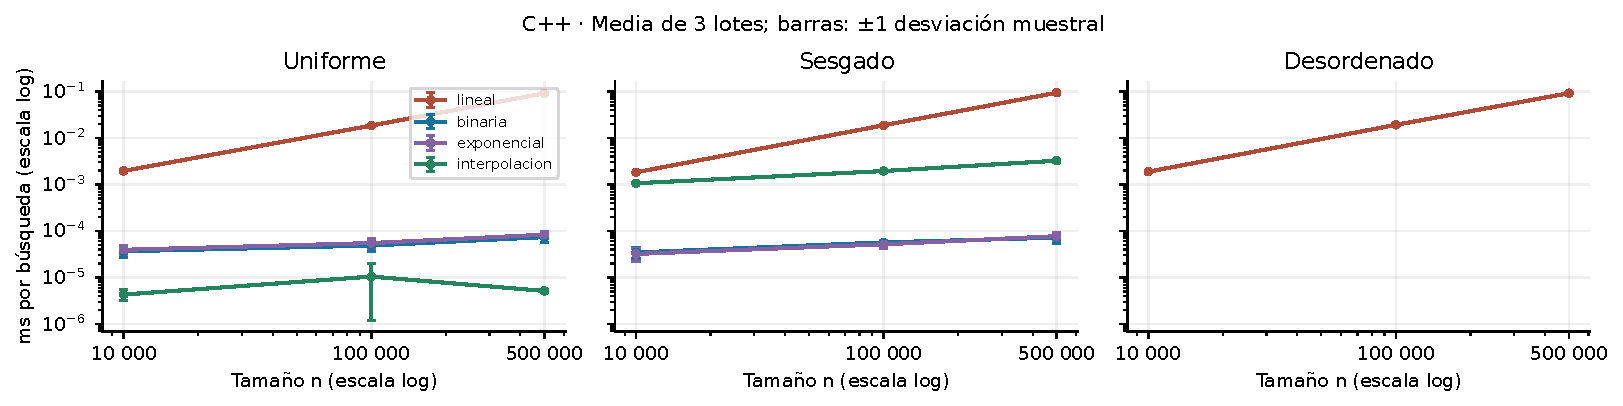
\includegraphics[width=\textwidth]{../graficos/tiempos_cpp.pdf}\par
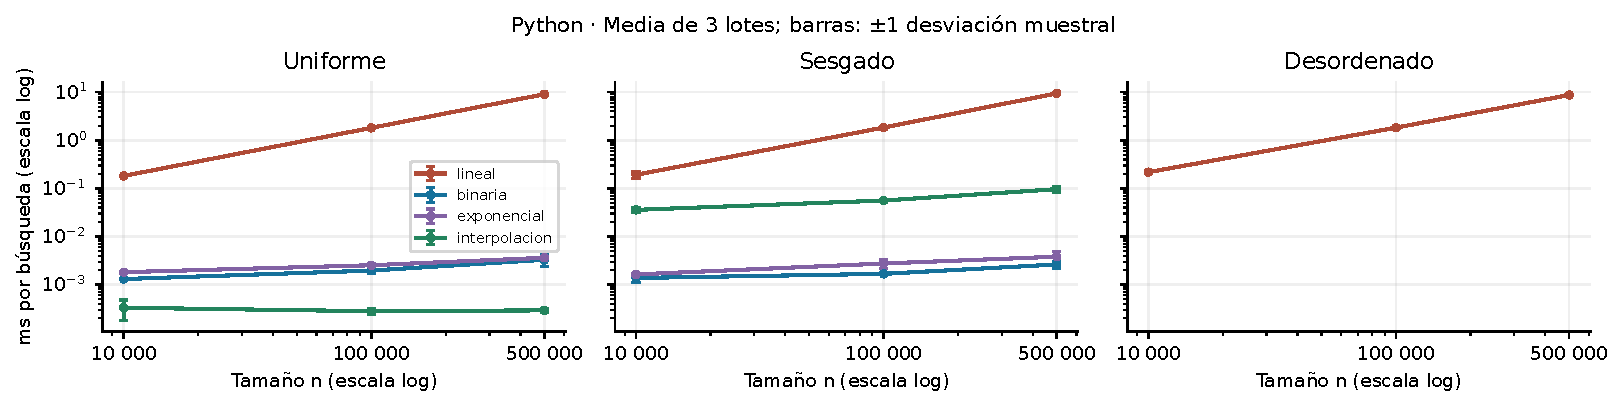
\includegraphics[width=\textwidth]{../graficos/tiempos_python.pdf}
\end{center}
\vspace{-6pt}
\textbf{Figuras 1 y 2.} Curvas generadas directamente desde los CSV; ambos ejes son logarítmicos. Las barras representan una desviación muestral entre lotes, no intervalos de confianza. Cada lenguaje tiene su propia escala vertical.

Al multiplicar $n$ por 50 en el uniforme, el tiempo lineal aumentó \CrecimientoLinealCpp{} veces en C++ y \CrecimientoLinealPy{} en Python: tendencia compatible con crecimiento lineal, con constantes y ruido reales. Para $n=500\,000$, binaria fue \VentajaBinariaCpp{} y \VentajaBinariaPy{} veces más rápida que lineal, respectivamente. Interpolación fue \VentajaInterpolacionCpp{} y \VentajaInterpolacionPy{} veces más rápida que binaria en el uniforme, pero tardó \PenalidadInterpolacionCpp{} y \PenalidadInterpolacionPy{} veces lo de binaria en el sesgado.

\textbf{Conteo independiente.} En C++, para el uniforme, lineal pasó de 6542.549 a 326242.621 comparaciones; binaria de 24.878 a 35.934 e interpolación permaneció en 3.4. En el sesgado de 500\,000, binaria registró 32.4 e interpolación 1600.14. Se cuentan comparaciones entre valores, incluidos límites y extremos; no controles de índices ni aritmética. El gráfico completo está en \texttt{graficos/comparaciones.pdf}. Los conteos respaldan la interpretación sin depender de milisegundos.
\newpage
\fontsize{9.5}{11}\selectfont
\section{Discusión: respuestas a las preguntas de la práctica}
\begin{enumerate}[label=\textbf{\arabic*.},itemsep=3pt]
\item \textbf{¿Por qué binaria supera a lineal en datos ordenados?} El orden permite descartar mitades. En el uniforme grande se obtuvieron unas 36 comparaciones frente a 326 mil de lineal. La menor cantidad de pasos compensa aquí el acceso menos secuencial de binaria.
\item \textbf{¿Cuándo interpolación puede superar a binaria?} Cuando valor y posición se relacionan aproximadamente de manera lineal. En nuestros enteros consecutivos la estimación es exacta; cada hit requiere una sola posición estimada. La media de 3.4 comparaciones incluye cuatro por hit y dos por miss externo.
\item \textbf{¿Cuándo pierde la ventaja?} Ante concentraciones, huecos grandes o valores extremos que distorsionan la estimación. El sesgado lo evidencia, sin llegar a demostrar el peor caso. Un arreglo $[0,1,\ldots,n-2,n^2]$ buscando $n-2$ puede provocar avances casi unitarios y costo lineal.
\item \textbf{¿Por qué afecta el sesgo?} El 80\% ocupa solo un rango numérico estrecho: la fracción de valores ya no representa la fracción de posiciones. La fórmula subestima posiciones en esa zona y necesita reiterar; binaria depende del orden, no de la uniformidad numérica.
\item \textbf{¿Para qué sirve exponencial con límite desconocido?} Duplica índices hasta superar la clave o detectar fin y luego refina con binaria. Requiere acceso indexado seguro; un flujo únicamente secuencial no permite saltos gratuitos. Aquí conocemos $n$: se estudia la acotación, sin simular una fuente infinita ni medir esa ventaja específica.
\item \textbf{¿Cómo influyen caché, localidad, ramas y constantes?} Lineal lee posiciones consecutivas, favorables a localidad y precarga; binaria salta y decide ramas dependientes de datos. Interpolación añade multiplicación y división. C++ usa enteros contiguos; Python maneja objetos y ejecuta bytecode. Son mecanismos plausibles (Van Sandt et al., 2019), no causas aisladas: no se midieron fallos de caché ni de predicción de ramas.
\item \textbf{¿Por qué Big O no predice milisegundos?} Omite constantes y términos menores; tampoco fija hardware, representación, distribución de consultas o carga del sistema. Exponencial y binaria comparten orden logarítmico y aun así difieren. Las pequeñas ventajas de exponencial en algunos conjuntos C++ no justifican un ganador universal, especialmente con la dispersión observada.
\end{enumerate}
\section{Heurística propuesta}
Se propone un selector sencillo, implementado y probado aparte en \texttt{python/heuristica.py}. Sea $q$ el número previsto de consultas y $E$ el error máximo entre posición relativa y valor normalizado, estimado con 33 posiciones equiespaciadas:
\begin{quote}\small
\textbf{Si} límite desconocido: exponencial con acceso seguro si hay orden certificado; si no, lineal hasta fin.\par
\textbf{Si} $n<64$: lineal. Si no hay certificado de orden, verificarlo una vez en $O(n)$.\par
\textbf{Si} desordenado: comparar $qn$ con $n\log_2n+q\log_2n$; ordenar una copia y usar binaria solo si se amortiza; en otro caso, lineal.\par
\textbf{Si} extremos iguales: binaria. En otro caso, muestrear y calcular
$E=\max_i\left|\frac{a[i]-a[0]}{a[n-1]-a[0]}-\frac{i}{n-1}\right|$.\par
\textbf{Si} $E\leq0.05$: interpolación; si no, binaria.
\end{quote}
Los umbrales 64 y 0.05 son propuestos, no calibrados. El muestreo no certifica orden ni garantiza velocidad. El costo de verificar, copiar y ordenar debe amortizarse; para una sola consulta sin metadatos puede convenir lineal directamente. El modelo supone constantes iguales y orienta una decisión, no demuestra optimalidad. Si se requieren índices originales, se preservan al ordenar pares.
\section{Conclusiones}
Binaria ofrece una opción estable para datos ordenados no uniformes; interpolación destacó en el caso consecutivo y perdió claramente con sesgo. Lineal evita preparación en desordenados y pocas consultas; exponencial aporta acotación cuando la interfaz admite saltos sin conocer el final. Los resultados son reproducibles desde archivos compartidos y coherentes con estas explicaciones, pero no demuestran cotas asintóticas ni se extrapolan a cualquier equipo o distribución.
\clearpage\section*{Referencias}
\addcontentsline{toc}{section}{Referencias}
\begingroup\fontsize{10}{12}\selectfont\setlength{\parskip}{8pt}
\newcommand{\referencia}[1]{\par\hangindent=1.27cm\hangafter=1 #1\par}
\referencia{Cormen, T. H., Leiserson, C. E., Rivest, R. L., \& Stein, C. (2022). \textit{Introduction to algorithms} (4th ed.). MIT Press. \url{https://mitpress.mit.edu/9780262046305/introduction-to-algorithms/}}
\referencia{Erickson, J. (2019). \textit{Algorithms}. \url{https://jeffe.cs.illinois.edu/teaching/algorithms/}}
\referencia{Google. (s.\,f.). \textit{User guide} [Documentación de Google Benchmark]. GitHub. Recuperado el 10 de septiembre de 2026, de \url{https://github.com/google/benchmark/blob/main/docs/user_guide.md}}
\referencia{Morin, P. (s.\,f.). \textit{Open data structures (in Python)}. Recuperado el 10 de septiembre de 2026, de \url{https://opendatastructures.org/ods-python/}}
\referencia{Perl, Y., Itai, A., \& Avni, H. (1978). Interpolation search---a log log N search. \textit{Communications of the ACM, 21}(7), 550--553. \url{https://doi.org/10.1145/359545.359557}}
\referencia{Python Software Foundation. (s.\,f.-a). \textit{Built-in types}. En \textit{Python 3.12 documentation}. Recuperado el 10 de septiembre de 2026, de \url{https://docs.python.org/3.12/library/stdtypes.html}}
\referencia{Python Software Foundation. (s.\,f.-b). \textit{random---Generate pseudo-random numbers}. En \textit{Python 3.12 documentation}. Recuperado el 10 de septiembre de 2026, de \url{https://docs.python.org/3.12/library/random.html}}
\referencia{Python Software Foundation. (s.\,f.-c). \textit{time---Time access and conversions}. En \textit{Python 3.12 documentation}. Recuperado el 10 de septiembre de 2026, de \url{https://docs.python.org/3.12/library/time.html}}
\referencia{Sedgewick, R., \& Wayne, K. (2011). \textit{Algorithms} (4th ed.). Addison-Wesley. \url{https://algs4.cs.princeton.edu/}}
\referencia{Skiena, S. S. (2020). \textit{The algorithm design manual} (3rd ed.). Springer. \url{https://doi.org/10.1007/978-3-030-54256-6}}
\referencia{Van Sandt, P., Chronis, Y., \& Patel, J. M. (2019). Efficiently searching in-memory sorted arrays: Revenge of the interpolation search? En \textit{Proceedings of the 2019 International Conference on Management of Data} (pp. 1791--1808). Association for Computing Machinery. \url{https://doi.org/10.1145/3299869.3300075}}
\referencia{Zanabria Galvez, A. H. (s.\,f.). \textit{Práctica 01 — Búsquedas y Notación Asintótica} [Guía de práctica, SIS210]. Universidad Nacional del Altiplano.}
\endgroup

\end{document}
